%\documentclass[14pt]{extarticle}
\documentclass[11pt]{article}
\usepackage{natbib}
\usepackage[dvipdfm,colorlinks=true,urlcolor=DarkBlue,linkcolor=DarkBlue,bookmarks=false,citecolor=DarkBlue]{hyperref}

\usepackage[pdftex]{graphicx}
\usepackage{fancyhdr}
\usepackage[T1]{fontenc}
\usepackage{palatino}
\usepackage[utf8]{inputenc}
%\usepackage[super]{nth}
\usepackage{setspace}
\usepackage{placeins}
\usepackage{subfigure}
\usepackage{multirow}
\usepackage{rotating}
\usepackage{marvosym}  % Used for euro symbols with \EUR
\newcommand{\HRule}{\rule{\linewidth}{0.5mm}}
\usepackage{longtable} %% Allows the use of the longtable format produced by xl2latex.rb
\usepackage{lscape} %% Allows landscape orientation of tables
\usepackage{appendix} %% Allows customization of the appendix properties
\setcounter{tocdepth}{1} %% Restricts the table of contents to the section header level entries only

\usepackage{geometry}
\geometry{letterpaper}
\usepackage{amsmath}
\usepackage[stable]{footmisc}

%% The following settings are for the listings environment in R
\usepackage{listings}
\usepackage[svgnames]{xcolor}
\usepackage{soul}
\sethlcolor{LightGoldenrodYellow}
\lstset{backgroundcolor=\color{LightYellow}}
\lstset{framextopmargin=6pt, framexbottommargin=6pt, framerule=4pt, rulecolor=\color{White}}

\title{Individual-level evidence of IT skill specialization and formation
  in the advanced industrial economies\thanks{DRAFT NOT FOR DISTRIBUTION}}
\author{Mark Huberty\thanks{Travers Department of Political Science,
    University of California, Berkeley. Contact:
    \url{markhuberty@berkeley.edu}.}}
\date{\today}

\graphicspath{{../figures/}}

\begin{document}

\maketitle
\doublespacing

\section{Introduction}
\label{sec:introduction}
 
I present new evidence of comparative patterns of specialization and
technology adoption in the advanced industrial economies. 

\section{Institutions and skill development}
\label{sec:inst-skill-devel}


Theories of comparative political economy predict that institutional
variation in the advanced industrial economies will create diverging
patterns of skill formation in workers, and in technology adoption and
exploitation among firms. The Varieties of Capitalism literature in
particular \citep{Hall:2001} makes two predictions about technology
and skills: first, that workers in more liberal economies
will adopt more general skills than their counterparts in coordinated
economies; and second, that firms in liberal economies will be more
likely to engage in radical innovation and adopt leading-edge
technology. 

These claims rest on an implicit microeconomic model of firm and
worker behavior. In more liberal economies, the lack of employment
protection laws means that workers must consider the possibility of
losing their jobs without recourse. Likewise, firms must consider that
workers who have no protection will feel little loyalty to any given
firm. In that context, both workers and firms will converge on an
equilibrium that values general skills--the workers, so that they can
easily find jobs at other firms, and the firms, so that workers are
easily replaced. Conversely, countries with strong employment laws
will tend to favor specific skills, because firms must extract high
value from employees that cannot be easily dismissed, and because
employees believe that investment in firm-specific skills will be
rewarded by long employment tenure. 

Empricially, the evidence used to support these claims has typically
relied on macro-level measures of skill formation, including
rates university versus vocational training, patenting rates across
different kinds of technology, and aggregate R\&D
spending.\footnote{For a full set of metrics, see
  \cite{hall2009varieties}.} But these metrics do not directly measure
worker-level behavior. Rather, they measure aggregate behavior at the
societal level, and may not adapt to new markets or sectors that have
different needs for employment.

\section{Pursuing new data for measurement}
\label{sec:data}

I exploit a new dataset on technology adoption and skill formation in
the information technology industry. That dataset provides
individual-level evidence of cross-sectional and intertemporal
patterns of skill formation among workers worldwide, and augments that
data with measures of expertise and evidence of patterns of worker
interaction. 

StackExchange represents a collection of community-created and
maintained internet sites that field questions and answers on topics related to information
technology. Begun in 2008 by Joel Spolsky and colleagues, it has grown
into one of the most comprehensive communities of technical
information in the world. As of 2011, it reported approximately
725,000 users, 1.2 million site visits per day, and 4.2 million separate
answers covering 82\%  of the 1.9 million submitted questions. It had grown from its initial site,
StackOverflow\footnote{In programming parlance, a stack overflow
  refers to a program condition in which memory usage exceeds
  memory allocation, causing a program crash. Hence StackOverflow is,
  in a sense, excess memory for humans.}, to sites covering everything
from programming to data security to cooking and philosophy. 

The format of StackExchange interactions can be stylized as follows: a
user poses a question and tags the question with metadata related to
the specific technologies or technological domains the question
pertains to. Other users respond to the question. Those responses, in
turn, are rated by respondents, the person who posed the original
question, and other community members, on the basis of accuracy,
solution elegance, and completeness. Questions and answers can be
retrieved by querying metadata, the user ID of the questioner or
answerer, and other boolean search terms. 

\begin{figure}[ht]
  \centering
  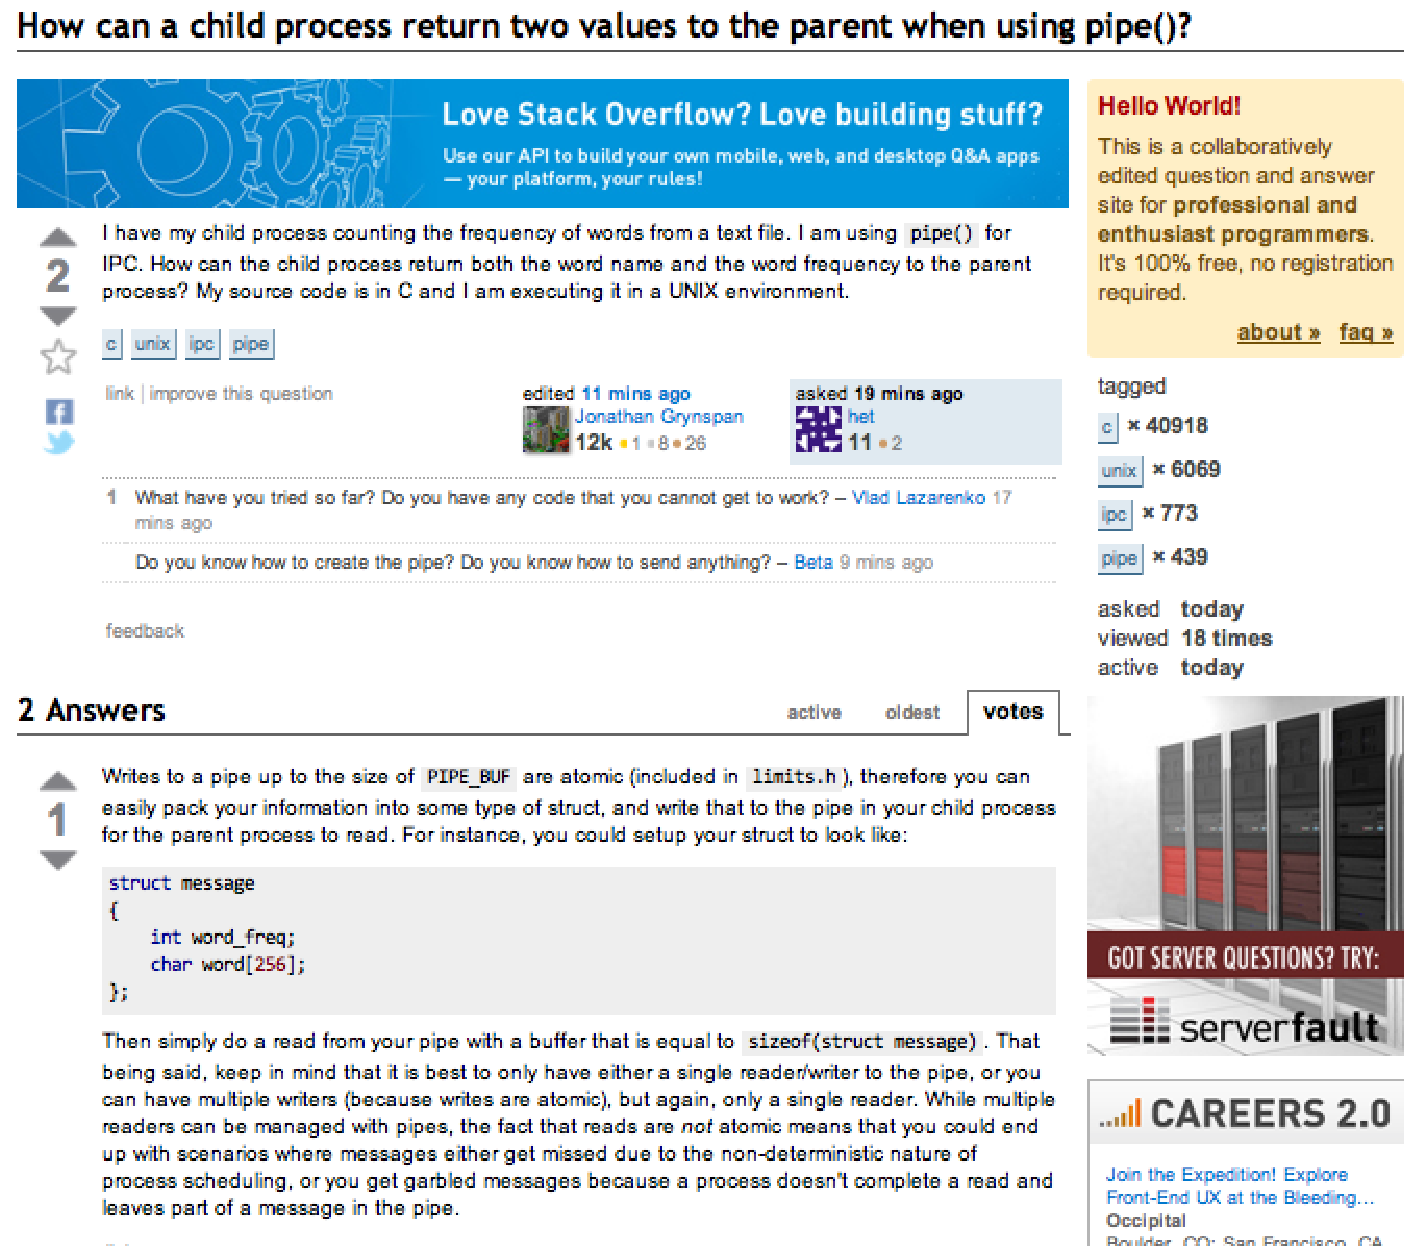
\includegraphics[width=\textwidth]{stack_question_answer}
  \caption{Sample StackOverflow question and answer}
  \label{fig:stack-question-answer}
\end{figure}

Users contribute to StackExchange through user accounts that contain a
range of information about the user. Users may, but are not required
to, provide information about their geographic location, interests,
website address, and other personal characteristics. There is no
evidence that this data is validated, and avatars or similarly
obscured or stylized user names and identities are permitted. 

%% Things to think about here: answered vs. unanswered questions;
%% multiple tags, community-modded responses, etc.

All StackExchange data is collected and published under a Creative
Commons license. In keeping with the license, StackExchange releases
a bi-monthly dump of its entire dataset, including the full record of
questions and answers, user profiles, record tagging and metadata, and
time stamps. The data are anonymized with respect to user names but
not other user metadata, including geographic location, web site,
the questions posed or answered by each user, and the
user's community-determined ``reputation''.\footnote{For more
  information on the StackExchange data dump, see
  \url{http://blog.stackoverflow.com/category/cc-wiki-dump/}. 
  %For information on how the data are rendered anonymous, see
  %\url{}. 
   For information
  on the terms of use for the Creative Commons license, see
  \url{http://creativecommons.org/licenses/}. For academic use of the
  data, including studies of social interaction and exchange markets,
  see \url{http://blog.stackoverflow.com/2010/05/academic-papers-using-stack-overflow-data/}.}

These data therefore represent a rich trove of information about the
interaction of IT workers worldwide. The dataset contains not only the location
and other information about the community members themselves, but also,
through the information on questions posed and answered and their reputation, the
kinds of technology they work with and are expert in, and their rating by
a community of their peers. As such, the data provide an opportunity
to directly observe patterns of specialization of knowledge and
interaction among IT workers across both countries and time. 

%% Hypotheses here, 

 


\section{Research Design}
\label{sec:research-design}

To employ the StackOverflow data in the study of skill and task
specificity, we first need to define exactly what is meant by the
terms task and skill, and how specificity will be defined. 

\subsection{Definitions}
\label{sec:definitions}

\subsubsection{Skill specificity}
\label{sec:skill-specificity}

\textbf{Skills} will refer to knowledge of the workings of specific
technologies, such as the $C$ or \textsc{scada} languages
themselves. Just as someone might be very knowledgeable about fuel
injection systems, but not necessarily ever need to rebuild them, so
could an IT worker be very knowledgeable about the $C$ programming
language without every using it to, say, optimize highly parallelized
programs used for scientific computing. Thus we should treat skill
separately from tasks. 

We may infer skill specificity from a question-and-answer site
like StackOverflow by analyzing the co-occurrance of technologies by
question. If questions about some technology often reference one or
many other technologies, we may infer that this technology is a more
\textit{general} technology than one for which questions ask about it
alone. Thus, for instance, the $C$ programming language is a
general-purpose technology used for everything from commercial
software development to scientific computing. In contrast, the
\textsc{scada} language is used predominately for control of
industrial machinery. 

To quantify this definition of specificity, we must first define the
relationship of technologies to each other. We can quantify this
relationship as the proximity between any two technologies in the
question space. Each question
$q_i, i \in [1...n]$ considers some technologies $T_q$, which are a subset of the entire set of technologies $T_Q$ considered in all
questions $Q$. The proximity between any two technologies $T_i$ and
$T_j$ $\in T_Q$ can be defined as the conditional
probability that they appear in questions together. Formally, $P(T_i
\in T_q | T_j \in T_q)$ can be defined as:

\begin{equation}
  \label{eq:1}
  p_{i,j} = \frac{\sum_{q \in Q} T_i \in T_q | T_j \in T_q}{\sum_{q \in Q} T_j \in T_q}
\end{equation}



\subsubsection{Task proximity}
\label{sec:task-specificity}

\textbf{Tasks} will refer to the application of
technologies. Consistent with the definition in equation \ref{eq:1},
we will begin to define task specificity by first defining task
proximity. Task proximity is the conditional probability of
co-occurrance of tasks in the question metadata. Thus, for instance, if questions regarding thread
optimization also deal with memory optimization, but rarely deal with
web page design, then we would regard thread and memory optimization
as more proximate tasks than thread optimization and web page design. Using the same notation as above, 

Each question
$q_i, i \in [1...n]$ considers some tasks $K_q$, which are a subset of the entire set of tasks $K_Q$ considered in all
questions $Q$. The proximity between any two tasks $K_i$ and
$K_j$ $\in K_Q$ can be defined as the conditional
probability that they appear in questions together. Formally, $P(K_i
\in K_q | K_j \in K_q)$ can be defined as:

\begin{equation}
  \label{eq:2}
  \frac{\sum_{q \in Q} K_i \in K_q | K_j \in K_q}{\sum_{q \in Q} K_j \in K_q}
\end{equation}

\subsubsection{From proximity to specificity}
\label{sec:from-prox-spec}

Scoring tasks or skills as more or less specific requires that we
translate from proximity between pairs of tasks or skills to a overall
measure of specificity. Given a proximity matrix $P$ that contains the
pairwise proximities $p_{i,j}$ between all technologies (skills) $T_i, T_j \in T_Q$, we may define the
specificity of any technology (skill) $T_i$ as in equation \ref{eq:3}, where
$\delta \in (0,1]$ is some threshold proximity value.

\begin{equation}
  \label{eq:3}
  ST_i = \sum_{q \in Q} p_{i,q} > \delta 
\end{equation}

Higher-valued $ST_i$ indicate skills that are more general, defined as
applied in concert with a larger set of other skills. We can write the
same relationship for task specificity $SK_i$.

Observers will note that some technologies (skills) are
heirarchical. For instance, the \texttt{bash} shell scripting
environment is a subset of the Unix operating system. Thus $P(unix |
bash)$ will be close to 1. In aggregate, leaving this fact unaccounted
for would simply reproduce heirarchies like this. To account for this
problem, we take the minimum of the pairwise conditional probabilities
for each skill or task pair. Thus while $P(Unix, bash)$ may be 1,
$P(bash, Unix)$ will most likely be far smaller, reflecting the fact
that only a portion of questions about Unix will inquire about the
\texttt{bash} environment.

\subsubsection{Individual-level skill and task specialization}
\label{sec:indiv-level-skill}

Given these definitions of task and skill specificity, we can now
define what we mean by those terms for any given individual. for a
user $u \in U$, their skill specificity is the mean specificity in all
questions $q \in Q$ that they have answered. Task specificity is
defined the same way. Each user thus receives both a skill and a task
specificity score. Conceptually, then, each user falls into one of
four possible categories: tackling specific tasks with general skills,
general tasks with general skills, specific tasks with specific
skills, or specific tasks with general skills. Notice, here, however,
that we are not bound by discrete categorization. Rather, we can
measure both task and skill specialization as continuous quantities.

\section{Results}
\label{sec:results}

\section{Discussion}
\label{sec:discussion}

\section{Conclusions}
\label{sec:conclusions}


\FloatBarrier
\bibliography{/bibs/VOC_Bib}
\bibliographystyle{apalike}
\end{document}